\section{Numerical checks}\label{app:checks}

\emph{Grid convergence.} Three operating points (Mackey--Glass, first series) were simulated on four grids, 512 or 1024 modes with 20
or 40 RK4IP steps per symbol, each with six new noise realisations; the results agree within the run-to-run spread of about 12\%.
An earlier apparent grid dependence of about 30\% came from the optimistic bias of selecting a point on one noise realisation, not
from the grid. The trained device of Section~\ref{sec:gradient} is the only result where the grid mattered more (14\% between 128 and
256 modes), which is why training uses at least 256 modes and every result is re-checked on 512.

\emph{Selection bias.} Choosing an operating point on one run and reporting the test error of that same run is optimistic by 10 to
30\% at the best points, and sharing one set of noise random numbers across series adds to this. All tables and figures therefore use
the protocol of Section~\ref{sec:protocol}: selection on the mean of three new pairs of runs, reporting on six further new pairs, with
independent noise per series; the software baselines are re-tested in the same way.

\section{Mask ablation}\label{app:ablation}

Figure~\ref{fig:ablation} shows the ablation of Section~\ref{sec:ablation} (realistic noise, 128 random operating points per variant,
the protocol of Section~\ref{sec:protocol}, three series). On both tasks the order is the same: random phases at equal amplitudes are
at least as good as the full mask, random amplitudes in phase are clearly worse, and the uniform comb is worst.

\begin{figure}[htbp]
\centering
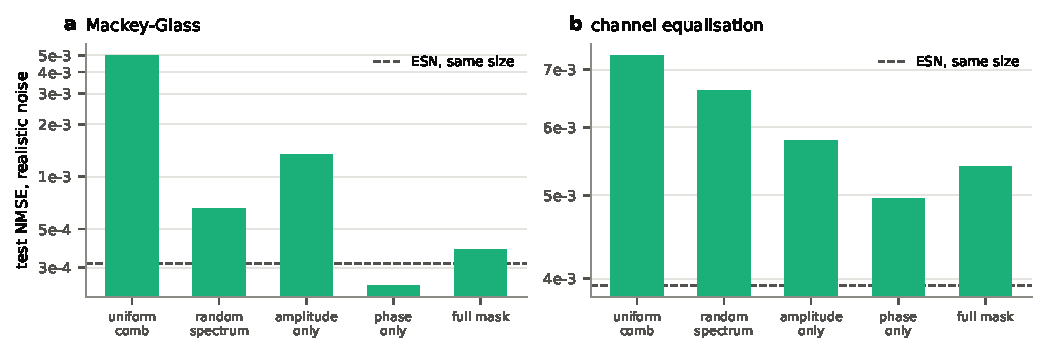
\includegraphics[width=\linewidth]{figS1_mask_ablation}
\caption{Mask ablation under realistic noise. Test error of the uniform comb, a random static spectrum with one common modulation
($w_\mu\propto b_\mu$), random amplitudes with all lines in phase, random phases at equal amplitudes, and the full mask; dashed: ESN
with the same readout dimension (input noise $3\times10^{-3}$). Bars: $\pm1$ relative standard deviation between pairs of new runs
(bars smaller than the marker are hidden).
The full mask gives $3.8\times10^{-4}$ in this batch ($3.3\times10^{-4}$ in Table~\ref{tab:encodings}). (a) Mackey--Glass;
(b) channel equalisation.}
\label{fig:ablation}
\end{figure}

\section{Fibre-link equalisation}\label{app:fibre}

As a realistic communication task we equalise a 28~GBd PAM-4 signal after 17~km of standard single-mode fibre with intensity
modulation and direct detection (chromatic dispersion, loss, Kerr nonlinearity, square-law detection and receiver noise), with 256
random operating points per encoding, the protocol of Section~\ref{sec:protocol} and test parts of 5000 symbols
(Fig.~\ref{fig:fibre}). NMSE and symbol error rate are: $2~\mathrm{ns}$ symbols $2.0\times10^{-2}$ and $1.6\times10^{-3}$; phase mask
$2.3\times10^{-2}$ and $2.3\times10^{-3}$; uniform comb $2.4\times10^{-2}$ and $3.7\times10^{-3}$; best single pump $3.7\times10^{-2}$ and
$1.6\times10^{-2}$; linear equaliser $2.5\times10^{-2}$ and $3.5\times10^{-3}$; ESN $1.8\times10^{-2}$ and $1.4\times10^{-3}$. The bit
error rate of $3.8\times10^{-3}$ commonly used as the hard-decision FEC threshold corresponds, for Gray-coded PAM-4, to a symbol error
rate of about $7.6\times10^{-3}$.
The mask and the readout-side changes beat the linear equaliser and the single-pump encoding but not the ESN (the $2~\mathrm{ns}$ group
is about 15\% worse). These resonators are treated at about 1~GBd, so the comparison is of equalisation capability, not of rate.
Operating the resonator at 28~GBd needs $Q\approx2\times10^{4}$ to $4\times10^{4}$, and with at most 1~W the Kerr effect is barely used:
Si$_3$N$_4$ reaches $2.3\times10^{-2}$ and $2.9\times10^{-3}$, silica $2.4\times10^{-2}$ and $3.2\times10^{-3}$, only about 15\% better than
the linear equaliser in symbol error rate. Without readout taps all encodings are poor here: the memory comes entirely from the taps.

\begin{figure}[htbp]
\centering
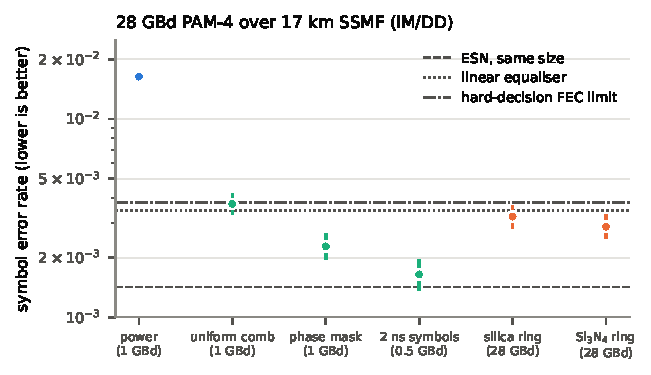
\includegraphics{figS2_fibre_link}
\caption{Symbol error rate on 28~GBd PAM-4 over 17~km of standard single-mode fibre (IM/DD). Blue: single-pump power encoding; green:
input combs processing the received samples offline at 1~GBd or 0.5~GBd (a test of equalisation capability, not of rate); orange:
low-$Q$ rings operated at the link rate (here orange does not denote soliton encodings as in Fig.~\ref{fig:encodings}). Bars: 95\%
Poisson intervals of the error count over 90\,000 symbols. Dashed: ESN with the same readout dimension; dotted: linear equaliser;
dash-dotted: symbol error rate corresponding to the hard-decision FEC threshold (bit error rate $3.8\times10^{-3}$, Gray-coded
PAM-4).}
\label{fig:fibre}
\end{figure}

\section{Closed-loop control}\label{app:closedloop}

The resonator predicts the next state of the Hénon map without control, and a bounded decision rule chooses the control from the
prediction. Two tasks are considered: tracking a commanded trajectory and holding the unstable fixed point. Predictors are compared with
a linear predictor, NG-RC, a 31-node ESN and the exact model; the three resonator variants are each chosen from 64 candidate points and
the ESN from 96.

With PIN detectors the tracking error on the first training record (eight trials, Fig.~\ref{fig:closedloop}b) is $1.0$ for the linear predictor, $7.0\times10^{-4}$ for the ESN,
$6.2\times10^{-3}$ for the plain mask, $2.3\times10^{-3}$ with stronger drop coupling and $4.4\times10^{-4}$ with $2~\mathrm{ns}$ symbols
($2.3\times10^{-5}$ without noise). Holding the unstable fixed point, the $2~\mathrm{ns}$ resonator stays stabilised 99.6\% of the time with
0.4 losses per thousand steps, the same as the exact model; the ESN reaches 99.5\% and 1.6, the plain mask 86\% and 97.
The decision quality is set by the prediction noise: the software predictors' error is set entirely by their input noise
(Fig.~\ref{fig:software}c), and below about $2.4\times10^{-3}$ (tracking) and $1.7\times10^{-3}$ (holding) the ESN and NG-RC are better
than the resonator; at $10^{-3}$ the ESN and NG-RC track with $8.6\times10^{-5}$ and $7.5\times10^{-5}$, about 5 times better.
Detuning jitter with the correlation of the main noise model (one symbol) up to 3\% leaves the $2~\mathrm{ns}$ resonator's tracking error between $4.2\times10^{-4}$ and $5.1\times10^{-4}$
(Fig.~\ref{fig:closedloop}c), but a slow drift (correlation time 1000 symbols) of 1\% makes it 2.4 times worse than the ESN and of 3\%
12 times worse; at 0.1\% and 0.3\% it is still better ($4.2\times10^{-4}$ and $5.6\times10^{-4}$ against $6.9\times10^{-4}$). Slow
detuning drift must therefore be locked to within about 0.3\% of the half-linewidth (about 0.4~MHz at this point). The ranking holds
over four training records with eight trials each (32 trials; mean tracking error of the $2~\mathrm{ns}$ resonator $4.5\times10^{-4}$)
but uses a single textbook map.

\begin{figure}[htbp]
\centering
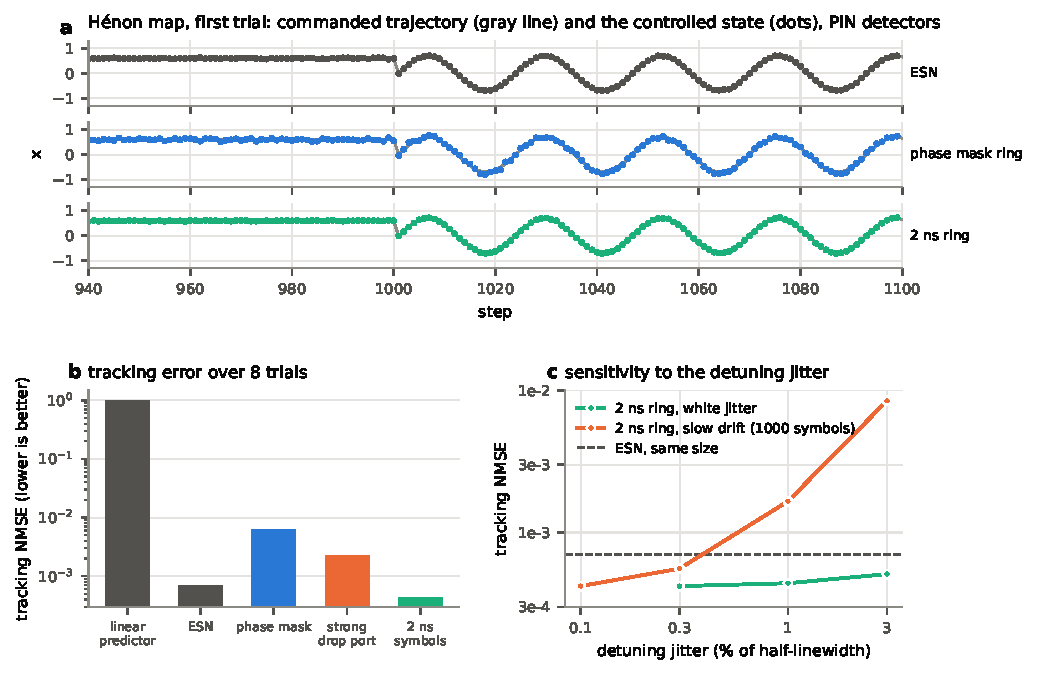
\includegraphics[width=\linewidth]{figS4_closed_loop}
\caption{Closed-loop tracking of the Hénon map with PIN detectors.
(a) First trial: commanded trajectory (grey line) and controlled state (dots) for the ESN, the plain phase-mask resonator and the
resonator with $2~\mathrm{ns}$ symbols. (b) Tracking error, pooled over the eight trials of the first training record (no spread
shown), for the linear predictor, the ESN and three resonator variants. (c) Tracking error of the $2~\mathrm{ns}$ resonator against detuning jitter with a
correlation time of one symbol (as in the main noise model) or a slow drift (correlation time 1000 symbols); dashed: ESN. Software
predictors receive input noise $3\times10^{-3}$ here.}
\label{fig:closedloop}
\end{figure}
